\chapter{JUSTIFICATIVA DE OFERTA DO CURSO}

A computação, inicialmente, foi definida como uma atividade que usa o computador para atingir seu objetivo ou meta. Na atualidade, a computação envolve diversas tecnologias com a finalidade de permitir a melhoria da qualidade de vida da sociedade. Assim, a ciência da computação engloba a construção e implementação de projetos de \textit{hardware} e \textit{software} para uma extensa gama de propósitos, processando, estruturando e administrando diversos tipos de sistemas de informação. Portanto, consiste em usar o computador para estudos científicos, construção de uma extensa variedade de tipos de sistemas computacionais, e por conseguinte, ajudar o desenvolvimento tecnológico da sociedade na busca do bem-estar social.

Na UFRPE, a história da Informática e Computação começa em 1999, quando o Curso de Licenciatura em Computação da UFRPE foi instituído e teve a primeira oferta de vestibular em 2000. Legalmente, o referido curso encontra-se Autorizado, segundo Resolução CEPE 265/1999, implantado segundo Resolução CUNI no. 181/99, e foi reconhecido junto ao MEC/INEP em novembro de 2005. O Projeto Pedagógico em vigor encontra-se homologado segundo Resolução CEPE de nº 220/2018. Em dezembro de 2006, foi avaliado pelo INEP/MEC, o qual recebeu o conceito CONDIÇÕES BOAS. O curso de Licenciatura em Computação foi criado pois havia, na UFRPE, poucos docentes da Área de Computação e a universidade possuía um consolidado Departamento de Educação. Assim, naquele momento, o perfil mais adequado foi o de Licenciatura em Computação. Neste cenário, existe na UFRPE, desde o ano 2000, a competência em Informática e Computação e, em 2005, seu quadro docente possuía 06 (seis) Doutores em Computação. Hoje, a Computação no Campus de Recife é composto por três cursos: o de Licenciatura em Computação como já citado, o de Bacharelado em Ciência da Computação e o de Bacharelado em Sistemas de Informação, bem como dois cursos de pós-graduação, o de Biometria e Estatística Aplicada que possui Mestrado e Doutorado e o curso de Informática Aplicada com Mestrado. 

A UFRPE, atualmente, possui também a Unidade Acadêmica de Educação à Distância e Tecnologia, ofertando os cursos de Licenciatura em Computação e Bacharelado em Sistemas de Informação em diversos polos espalhados no Nordeste, bem como com projetos de pesquisa aprovados na FACEPE. O curso de Licenciatura em Física foi o primeiro projeto de curso na modalidade a distância que foi aprovado conforme a Portaria nº 3.726 em 21/10/2005, publicada em 24/10/05 do DOU.

Em face deste contexto e pela expertise adquirida durante estes anos, a UFRPE sentiu-se confortável para a criação do Curso de Bacharelado em Ciência da Computação no município de Garanhuns/PE. A primeira turma teve sua entrada em 2009 e foi concluída em 2013. 

O curso de BCC da UAG foi criado em 2008, sob o Art. 35 Decreto 5.773/06 (Redação dada pelo Art. 2 Decreto 6.303/07), com o Projeto Pedagógico do Curso inicial (Proc. nº 014727/2008, de 01/08/2008) em seguida sofrendo reformulação (Proc. nº 018649/2011, de 11/11/2011). O curso foi reconhecido sob a portaria do MEC nº. 649, de 10/12/2013, DOU nº. 240, Seção 1, 11/12/2013, ISSN 1677-7042. p. 25-26.

A UAG está situada no Município de Garanhuns, segundo maior da Mesorregião do Agreste Meridional pernambucano, com área de 458.552 km$^2$, população de 138.983 habitantes (IBGE, 2018) e encontra-se a cerca de 230 km da capital Recife, onde fica a Reitoria da UFRPE.

\section{Contexto de inserção do curso na região}

Além de se configurar como área de entroncamento viário, o Município de Garanhuns centraliza, economicamente, parte da Região Agreste, denominado Agreste Meridional, composta por esse e outros 26 municípios. Devido à  localização  e  à  sua  importância como polo regional, Garanhuns, historicamente, esteve marcada por sua vocação e perfil atrativo às atividades de comércio e serviços, especialmente ligados às áreas de educação, saúde e turismo.

Segundo a Agência CONDEPE/FIDEM (2017), a rede de influência de Garanhuns é constituída pelos municípios que estão no entorno da microrregião de Garanhuns e, também, aponta a centralidade da cidade que se consolida como importante polo comercial e de serviços para o qual se direcionam populações vindas de municípios situados no Agreste Meridional, Central e na Mata Sul, conforme pode ser visto na Figura~\ref{fig:centralidade}.


\begin{figure}[!htb]
    \centering
    \caption{\label{fig:centralidade}Centralidade, Área de Influência e Equipamentos Urbanos de Garanhuns}
    
    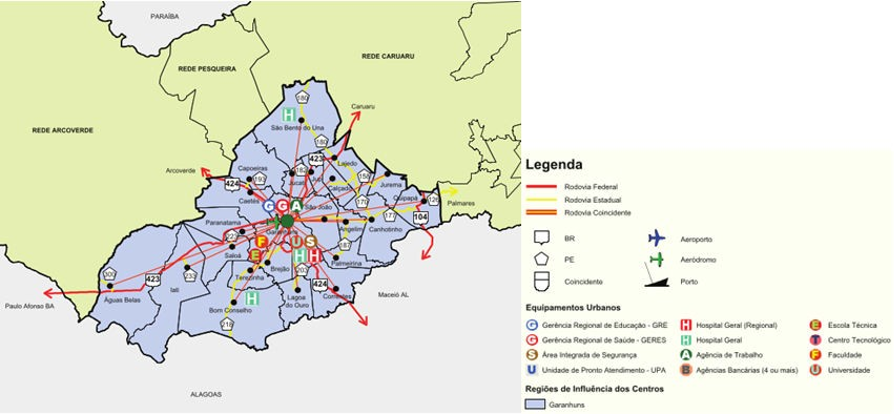
\includegraphics[width=\textwidth]{images/centralidade.png}
    \nota[Fonte]{Agência CONDEPE/FIDEM (2017)}
\end{figure}


A cidade de Garanhuns funciona como uma rede primaz, onde não há outros pólos de influência à sua proximidade. Essa rede urbana compreende 7,49\% do território estadual e influencia diretamente 12,43\ dos municípios pernambucanos. O que representa 3,57\% do PIB do Estado, onde o núcleo (Garanhuns) representa 33,57\% do PIB da rede (CONDEPE/FIDEM, 2017).

A ideia de criar um curso na área de computação existiu desde a concepção da Unidade Acadêmica de Garanhuns em setembro de 2005, quando começaram a funcionar 4 (quatro) cursos de graduação: Agronomia, Licenciatura Normal Superior (transformada no curso de Licenciatura em Pedagogia), Medicina Veterinária e Zootecnia. Em reunião geral, ocorrida em dezembro de 2007, ficou decidido em processo de votação que seria proposta a criação de 3 (três) novos cursos dentro do processo de Reestruturação Universitária (REUNI). Entre eles foi indicado o curso de Bacharelado em Ciência da Computação (BCC), no turno noturno, com o objetivo tanto de suprir a necessidade de um curso na área de computação, quanto proporcionar o desenvolvimento acadêmico da Universidade mediante uma forte interação com os demais cursos de graduação da UAG.

Além de interagir com as demais áreas da UAG, o curso de Bacharelado em Ciência da Computação veio atender a uma demanda regional identificada junto ao poder público local e à população. Portanto, o curso foi inserido dentro do contexto dos demais cursos da área de computação da UFRPE, de forma a contribuir com o desenvolvimento da UAG e dentro da realidade local. Para tanto, foram definidas áreas de atuação dos profissionais do curso bem como áreas de conhecimento que pudessem ser utilizadas para as outras áreas de conhecimentos já existentes na realidade da UAG-UFRPE.

De forma paralela, ressaltando a importância da  expansão  tecnológica,  constata-se que o uso do computador deixou de ser um diferencial para se tornar necessidade fundamental, tanto no contexto profissional quanto no dia a dia das pessoas. O advento da Internet transformou as tecnologias em elemento chave na construção da chamada sociedade da informação, modificando inclusive a forma de relacionamento na sociedade moderna. Dados de 2016 demonstram que existem no mundo cerca de 3.9 bilhões de usuários da Internet (ITU, 2018), e no Brasil a rede atende a aproximadamente 122 milhões de usuários.

O Brasil sofre com graves problemas tanto no acesso da população aos recursos computacionais quanto nas desigualdades regionais. Junto com a Internet surgem novas oportunidades de desenvolvimento ligadas à produção de conteúdo para a rede, aliados ao desenvolvimento de sistemas que usam grande quantidade de dados. Neste aspecto, é urgente a formação de profissionais ligados ao desenvolvimento de software. Nesse contexto, em 2006, a Sociedade Brasileira de Computação (SBC) definiu cinco grandes desafios atuais da computação:

\begin{enumerate}
    \item Gestão da informação em grandes volumes de dados multimídia distribuídos;
    \item Modelagem computacional de sistemas complexos artificiais, naturais, socioculturais e da interação homem-natureza;
    \item Impactos na computação da transição do silício para novas tecnologias;
    \item Acesso participativo universal do cidadão brasileiro ao conhecimento; e
    \item Sistemas disponíveis, corretos, seguros, escalonáveis, persistentes e ubíquos.
\end{enumerate}
	
Dentro desses desafios, pode-se contextualizar o curso de BCC da UAG em uma região carente de profissionais na área de desenvolvimento de software. Além disso, há o fato de haver, nessa região, claras possibilidades de aproveitamento dos profissionais a serem formados no ensino superior ofertado em Garanhuns. Com isso, obtêm-se a participação sócio-econômica dos atuais egressos das diferentes áreas técnicas científicas e informacionais (bacharéis, licenciados) em diversos municípios da região.

Adicionalmente, a região onde se encontra a UAG tem uma economia com base na agropecuária, e o município de Garanhuns tem uma forte atuação no setor de serviços, com forte apelo para o uso da Computação. Assim, a Computação é também um dos eixos norteadores do desenvolvimento municipal pelo fato do programa de expansão das universidades federais centrar-se na possibilidade de responder às demandas regionais sem, no entanto, restringir-se apenas à região, mas produzindo e transferindo conhecimentos, que é função inerente a toda Universidade.

Portanto, o curso de Bacharelado em Ciência da Computação foi projetado com eixos fundamentados em áreas do conhecimento que viessem a contribuir no desenvolvimento regional.

\section{Resultados Obtidos}

Em dezembro de 2015, o curso de Bacharelado em Ciência da Computação da UAG/UFRPE obteve a nota máxima de avaliação do ENADE (Exame Nacional de Desempenho dos Estudantes), ou seja, conceito 5. Isso fortalece a qualidade do desempenho dos estudantes com relação aos conteúdos programáticos previstos na diretriz curricular do curso, bem como o desenvolvimento de competências e habilidades necessárias ao aprofundamento da formação geral e profissional, e o nível de atualização dos estudantes com relação à realidade brasileira e mundial.

O curso de BCC foi avaliado com 4 estrelas (máximo de 5), sendo considerado Muito Bom nas duas últimas edições da Avaliação de Cursos Superiores do Guia do Estudante (GE), da Editora Abril em 2017 e 2018. Essa avaliação consta na publicação GE Profissões Vestibular 2018 e 2019.

O curso hoje é formado por 30 professores com dedicação exclusiva, distribuídos por formação e atuação nas principais áreas de conhecimento da Ciência da Computação, sendo aproximadamente 25 doutores e 5 mestres (doutorandos). Além disso, também contamos com professores das áreas de Matemática e Física. Atualmente o curso concorre e costumeiramente é contemplado com bolsas para projetos de pesquisa, extensão e iniciação tecnológica, como também possui grupos de pesquisa que tem gerado diversos artigos publicados por meio de trabalhos realizados com os discentes. Além de artigos, o curso promove melhorias na região por meio dos projetos de extensão que atende a diversas áreas, como projetos interdisciplinares em parceria com os outros cursos. Podemos citar alguns projetos, como: o desenvolvimento de aplicativos móveis para auxiliar agricultores e agrônomos nos processos de mecanização agrícola e para o ensino de química básica e avançada; soluções inteligentes para automatizar a irrigação de pequenos produtores rurais da região; ensino de programação básica para alunos de nível médio; e ensino de informática básica para a terceira idade.

O Centro de Tecnologia da Informação do Agreste Meridional de Pernambuco (Time JR.) é a Empresa Júnior do curso de Bacharelado em Ciência da Computação da UAG/UFRPE. A Time JR. é uma empresa formal composta por discentes de BCC, sob a orientação dos docentes, atuando como desenvolvedora de soluções para as diversas áreas do conhecimento e demanda da sociedade, atuando desde 2012 na região. 

Tomando por base o potencial criador e criativo que a conjuntura local oferece, como curso de Ciência da Computação, demais cursos e sociedade como um todo, e claro, da imensa demanda institucional e local represada, dois projetos foram criados para atuarem nesse cenário, o primeiro se refere a um Laboratório de Pesquisa e Desenvolvimento, chamado de BCC Coworking\footnote{\url{http://bcc.uag.ufrpe.br/bcccoworking}}, que é uma iniciativa exclusiva do curso de Computação, que surgiu com o propósito de servir como um local propício para o desenvolvimento de projetos reais, servindo até como fomento, com supervisão de profissionais da área, garantindo o conhecimento e a experiência técnica, através do uso de práticas e ferramentas do mercado de trabalho. É um ambiente onde o discente tem a oportunidade trazer sua ideia/projeto, de criar, manter e aumentar o \textit{networking} com outras pessoas de diversas áreas. É um local para aperfeiçoamento da produtividade. É importante destacar que não se trata de um espaço físico apenas, é principalmente um ambiente destinado aos estudantes em busca de conhecimento, experiência técnica, autonomia, fomentação e desenvolvimento de projetos. 

O segundo, diz respeito ao Laboratório Multidisciplinar de Tecnologias Sociais\footnote{\url{http://lmts.uag.ufrpe.br/}} (LMTS), como um espaço permanente de ensino, pesquisa, inovação tecnológica, extensão e de colaboração com a gestão institucional, contando com colaboradores da área técnica, mas também das demais áreas citadas, sejam eles, professores, técnicos ou estudantes. Este espaço agrega esta inteligência coletiva e as múltiplas iniciativas em curso ou idealizadas em prol especificamente para o desenvolvimento de \textit{softwares} livres ou públicos para atender as demandas da UFRPE e da sociedade em geral. O referido laboratório funciona com um propósito sem fins lucrativos, diferentemente da Time JR. (supracitada) e do BCC Coworking.

Atualmente, no contexto do curso de Ciência da Computação desta instituição, existem 7 (sete) grupos de pesquisa, liderados e coordenados por professores do curso. Estes grupos atuam nas grandes áreas da computação (Engenharia de Software, Inteligência Artificial, Banco de Dados, Redes de Computadores e Sistemas Distribuídos, Informática e Educação, entre outras) e desenvolvem atividades de pesquisa, monitoria, ensino e extensão.

\section{Categorias de cursos da área de computação e informática}

Com as diretrizes curriculares de 1999, foi criada a denominação da área de computação e informática orientando a elaboração do projeto político pedagógico dentro do tipo de curso escolhido. Assim, foram limitadas as possibilidades de nomes de cursos dessa área a 05 (cinco) tipos: Bacharelado em Ciência da Computação, Engenharia da Computação, Bacharelado em Sistemas da Informação, Cursos de Licenciatura em Computação e Cursos Superiores Tecnológicos, e posteriormente, o de Engenharia de Software. Segundo as diretrizes, esses cursos se enquadram em 04 (quatro) categorias básicas:

\begin{enumerate}
    \item Cursos que têm a computação como atividade-fim: Ciência da Computação e Engenharia da Computação;
    \item Cursos que têm a informática como atividade-meio:  Sistema da Informação;
    \item Cursos voltados para o ensino da informática: Licenciatura em Computação; e,
    \item Cursos Tecnológicos e sequenciais.
\end{enumerate}

Para que o curso escolhido se inserisse melhor dentro do desenvolvimento da UAG, optou-se pelo curso de Bacharelado em Ciência da Computação (BCC) que se enquadra na categoria de curso com a computação como atividade-fim.

O curso de BCC da UAG foi idealizado a partir do currículo de referência formulado em documento de 2005 pela IEEE Computer Society (Instituto de Engenheiros Eletricistas e Eletrônicos), e levando em conta as tendências e desafios para a área de informática descrita em publicação sobre a trajetória dos cursos de graduação da área de computação e informática publicada pela Sociedade Brasileira de Computação (SBC). A matriz curricular foi construída a partir do estudo de projetos de cursos de outras Instituições de Ensino Superior, de alto nível, seguindo as recomendações do Currículo de Referência da Sociedade Brasileira de Computação (1999) e as diretrizes de 2012 e 2016 do MEC.

Este Projeto Pedagógico vem sendo construído e revisado desde o final de 2015, com encontros mensais por parte do NDE, sendo inicialmente os encontros com todo o quadro docente do curso, com intuito de um planejamento mais robusto, que se tornasse duradouro. A partir de 2016 com reuniões mensais, uma proposta mais robusta foi sendo consolidada. Essa proposta no decorrer dos anos vem sendo continuamente ajustada e atualizada pelos membros do NDE. Entre as várias dificuldades encontradas pelo NDE para dar prosseguimento ao projeto, as principais foram, realizar um estudo mais profundo para entender e embasar a decisão do curso de se tornar vespertino, como também, mudanças nas resoluções da Sociedade Brasileira da Computação e do Ministério da Educação. E, do ano de 2018 em diante, sofrendo as adequações exigidas pelas Pró-reitoria de Ensino e Graduação, tendo essa pró-reitoria também enfrentado mudanças nesse período na abordagem de construção dos PPCs.
